\documentclass[11pt]{article}
% Compiler avec XeLaTeX (texte copiable, accents Unicode)
\usepackage{fontspec}
\usepackage{polyglossia}
\setdefaultlanguage{french}
\usepackage[margin=2.2cm]{geometry}
\usepackage{amsmath,amssymb}
\usepackage{graphicx}
\graphicspath{{images/}}
\usepackage{booktabs}
\usepackage{array}
\usepackage{enumitem}
\usepackage[hidelinks]{hyperref}
\usepackage{fancyvrb}
\setlength{\parskip}{0.3em}\setlength{\parindent}{0pt}

\title{IFT3295 -- TP1 : Assemblage de séquences\\\large Réponses aux questions écrites}
\author{Toky Erick Rabenantoandro (20266409)}
\date{9 octobre 2026}

\begin{document}
\maketitle


\setlist{nosep,leftmargin=*}
\section*{1. Chevauchement de séquences}
On note $v=X_i$ la séquence en lignes (taille $m$) et $w=X_j$ la séquence en colonnes (taille $n$).
Le score d'une colonne d'alignement est $\delta(a,b)=+4$ si $a=b$, $-4$ si $a\neq b$, et $-8$ pour un indel.
$V(i,j)$ est le meilleur score d'un alignement entre un suffixe de $v[1..i]$ et le préfixe $w[1..j]$.

\subsection*{Q1. Différence avec l'alignement global}
Dans l'alignement global, on aligne les deux séquences au complet, donc les indels au début et à la fin sont
pénalisés comme les autres. Pour un chevauchement, on veut seulement aligner la fin de $v$ avec le début de $w$
(alignement suffixe-préfixe). Le début de $v$ et la fin de $w$ ne font pas partie du chevauchement : ils ne
doivent donc pas être pénalisés.

\subsection*{Q2. Première ligne et première colonne}
\[ V(i,0)=0 \ \ \forall i \qquad\qquad V(0,j)=-8\,j \ \ \forall j \]
\begin{itemize}
\item Première colonne : le chevauchement peut commencer n'importe où dans $v$. Sauter le préfixe $v[1..i]$ ne
coûte rien, donc on met 0 (comme un « parcours gratuit » en alignement local).
\item Première ligne : le chevauchement doit commencer au premier caractère de $w$. Si on a déjà utilisé $j$
caractères de $w$ sans aucun caractère de $v$, ce sont forcément $j$ indels, donc $-8j$.
\end{itemize}

\subsection*{Q3. Relations de récurrence}
Pour $1\le i\le m$ et $1\le j\le n$, on prend le meilleur des trois cas habituels :
\[
V(i,j)=\max\begin{cases}
V(i-1,j-1)+\delta(v_i,w_j) & v_i \text{ aligné avec } w_j\\
V(i-1,j)-8 & v_i \text{ aligné avec un indel}\\
V(i,j-1)-8 & w_j \text{ aligné avec un indel}
\end{cases}
\]
C'est la même récurrence que pour l'alignement global : seules l'initialisation et la case finale changent.
On garde aussi, pour chaque case, un pointeur vers le cas choisi. La table se remplit ligne par ligne en $O(mn)$.

\subsection*{Q4. Retrouver l'alignement}
\begin{enumerate}
\item Le chevauchement doit finir à la fin de $v$, donc on regarde la dernière ligne. On choisit
$j^*=\arg\max_j V(m,j)$ ; le score du chevauchement est $V(m,j^*)$. S'il est $\le 0$, il n'y a pas de chevauchement.
\item On part de la case $(m,j^*)$ et on suit les pointeurs : diagonale $\Rightarrow$ on aligne $v_i$ avec $w_j$ ;
haut $\Rightarrow$ $v_i$ avec « - » ; gauche $\Rightarrow$ « - » avec $w_j$.
\item On s'arrête quand $j=0$ : tout le préfixe de $w$ a été aligné et le reste de $v$ est ignoré.
\item Comme on a construit l'alignement à l'envers, on l'inverse. La longueur du chevauchement est le nombre de
colonnes de l'alignement.
\end{enumerate}

\subsection*{Q5. Implémentation}
L'algorithme est dans \texttt{overlap.py} (\texttt{chevauchement\_maximal}), en $O(|X_i||X_j|)$.
Pour les deux premiers reads de \texttt{reads.fq}, on obtient un score de 8, l'alignement \texttt{TTAG}/\texttt{CTAG}
et un chevauchement de longueur 4.

\section*{2. Assemblage de fragments}
\subsection*{2.1 Matrice des scores}
La case (ligne $R_i$, colonne $R_j$) donne le score du chevauchement entre la fin de $R_i$ et le début de $R_j$.
La matrice n'est pas symétrique et sa diagonale est nulle. Les scores $\ge 80$ sont en gras.
\begin{table}[h]\centering
\resizebox{\textwidth}{!}{%
\begin{tabular}{c|rrrrrrrrrrrrrrrrrrrr}
$R_i \backslash R_j$ & 1 & 2 & 3 & 4 & 5 & 6 & 7 & 8 & 9 & 10 & 11 & 12 & 13 & 14 & 15 & 16 & 17 & 18 & 19 & 20 \\ \hline
\textbf{1} & 0 & 8 & 8 & 0 & 4 & 12 & 12 & 16 & 4 & \textbf{804} & 20 & 4 & 0 & 4 & \textbf{396} & 4 & 20 & \textbf{652} & 12 & \textbf{608} \\
\textbf{2} & 4 & 0 & 8 & 12 & 44 & 8 & 4 & \textbf{416} & 8 & 12 & \textbf{424} & 16 & 0 & \textbf{1060} & 12 & 12 & 12 & 8 & 4 & 0 \\
\textbf{3} & \textbf{396} & 12 & 0 & 24 & \textbf{1016} & 16 & 48 & 0 & 36 & \textbf{128} & 4 & 20 & 40 & 8 & 20 & 20 & 16 & 8 & 8 & 8 \\
\textbf{4} & 28 & 8 & 28 & 0 & 12 & \textbf{640} & \textbf{1024} & 16 & \textbf{1068} & 12 & 12 & \textbf{220} & 16 & 24 & 12 & \textbf{656} & \textbf{152} & 16 & 8 & 16 \\
\textbf{5} & \textbf{500} & 4 & \textbf{696} & 28 & 0 & 24 & 52 & 8 & 52 & \textbf{208} & 16 & 20 & 36 & 4 & 8 & 24 & 36 & 64 & 4 & 12 \\
\textbf{6} & 52 & 4 & 4 & 16 & 0 & 0 & 4 & 4 & 12 & 28 & 4 & 16 & 4 & 0 & 28 & 8 & \textbf{672} & 16 & 12 & 20 \\
\textbf{7} & 32 & 12 & 32 & \textbf{648} & 16 & \textbf{720} & 0 & 4 & \textbf{772} & 12 & 12 & 24 & 24 & 24 & 24 & \textbf{176} & \textbf{232} & 12 & 4 & 0 \\
\textbf{8} & 8 & 12 & \textbf{644} & 4 & \textbf{540} & 16 & 8 & 0 & 8 & 4 & \textbf{944} & 12 & 4 & 12 & 0 & 4 & 8 & 36 & 4 & 16 \\
\textbf{9} & 36 & 12 & 20 & \textbf{956} & 16 & \textbf{668} & \textbf{1044} & 4 & 0 & 8 & 4 & 64 & 12 & 24 & 20 & \textbf{492} & \textbf{196} & 8 & 4 & 12 \\
\textbf{10} & 4 & 0 & 0 & 8 & 32 & 8 & 8 & 24 & 12 & 0 & 32 & 4 & 12 & 12 & \textbf{640} & 4 & 8 & \textbf{904} & \textbf{184} & \textbf{868} \\
\textbf{11} & 20 & 20 & \textbf{620} & 4 & \textbf{524} & 12 & 12 & \textbf{1072} & 4 & 12 & 0 & 24 & 28 & 24 & 8 & 8 & 16 & 20 & 12 & 12 \\
\textbf{12} & 28 & 28 & 48 & \textbf{900} & 16 & \textbf{460} & \textbf{820} & 0 & \textbf{856} & 4 & 16 & 0 & 28 & 24 & 16 & \textbf{996} & 20 & 16 & 8 & 4 \\
\textbf{13} & 68 & 32 & 32 & \textbf{744} & 24 & \textbf{272} & \textbf{656} & 0 & \textbf{692} & 16 & 8 & \textbf{860} & 0 & 36 & 16 & \textbf{848} & 32 & 24 & 4 & 28 \\
\textbf{14} & 16 & \textbf{756} & 12 & 12 & 52 & 20 & 8 & \textbf{452} & 12 & 16 & \textbf{492} & 16 & 8 & 0 & 4 & 12 & 20 & 16 & 8 & 16 \\
\textbf{15} & 20 & 8 & 28 & 12 & 16 & 12 & 16 & 12 & 8 & 4 & 12 & \textbf{80} & \textbf{260} & 28 & 0 & 28 & 20 & 24 & \textbf{632} & 24 \\
\textbf{16} & 20 & 16 & 24 & \textbf{1032} & 16 & \textbf{552} & \textbf{944} & 12 & \textbf{988} & 8 & 20 & \textbf{692} & 8 & 20 & 12 & 0 & \textbf{80} & 12 & 8 & 8 \\
\textbf{17} & 16 & 4 & 32 & 16 & 16 & 32 & 8 & 12 & 4 & 24 & 20 & 12 & 4 & 28 & 12 & 8 & 0 & 16 & 8 & 20 \\
\textbf{18} & 16 & 0 & 8 & 12 & 8 & 4 & 4 & 8 & 8 & \textbf{240} & 16 & 8 & 4 & 16 & \textbf{808} & 8 & 4 & 0 & \textbf{368} & \textbf{1004} \\
\textbf{19} & 48 & 20 & 16 & \textbf{388} & 8 & 20 & \textbf{316} & 8 & \textbf{368} & 16 & 20 & \textbf{520} & \textbf{732} & 16 & 24 & \textbf{492} & 20 & 20 & 0 & 4 \\
\textbf{20} & 8 & 4 & 0 & 4 & 0 & 8 & 4 & 0 & 0 & 0 & 4 & 0 & 64 & 8 & \textbf{908} & 4 & 16 & \textbf{644} & \textbf{428} & 0 \\
\end{tabular}}
\end{table}

\subsection*{2.2a Effet du seuil de 80}
Sans seuil, presque toutes les paires de reads ont un petit score positif, parce que quelques bases peuvent se
ressembler par hasard : le graphe est presque complet et inutilisable. Le seuil de 80 enlève ces faux
chevauchements et ne garde que les arêtes entre reads qui se recouvrent vraiment. Le graphe devient beaucoup plus
simple, mais il contient encore des arêtes redondantes (transitives) et des cycles de deux noeuds, qu'il faut
enlever à l'étape suivante.

En chiffres (calculés sur \texttt{overlap\_matrix.csv}) : sans seuil, 360 paires ont un score positif ; avec le
seuil, il reste 76 arêtes. Le plus grand score éliminé est 68, alors que les chevauchements gardés dans l'ordre
final valent tous au moins 492. Il reste 13 cycles de deux noeuds.

La figure ci-dessous montre le graphe filtré (seuil $\ge 80$). Elle a été générée à partir du fichier
\texttt{graphe.dot} produit par \texttt{main.py}, avec le site GraphvizOnline
(\url{https://dreampuf.github.io/GraphvizOnline}, moteur \texttt{dot}).
\begin{center}
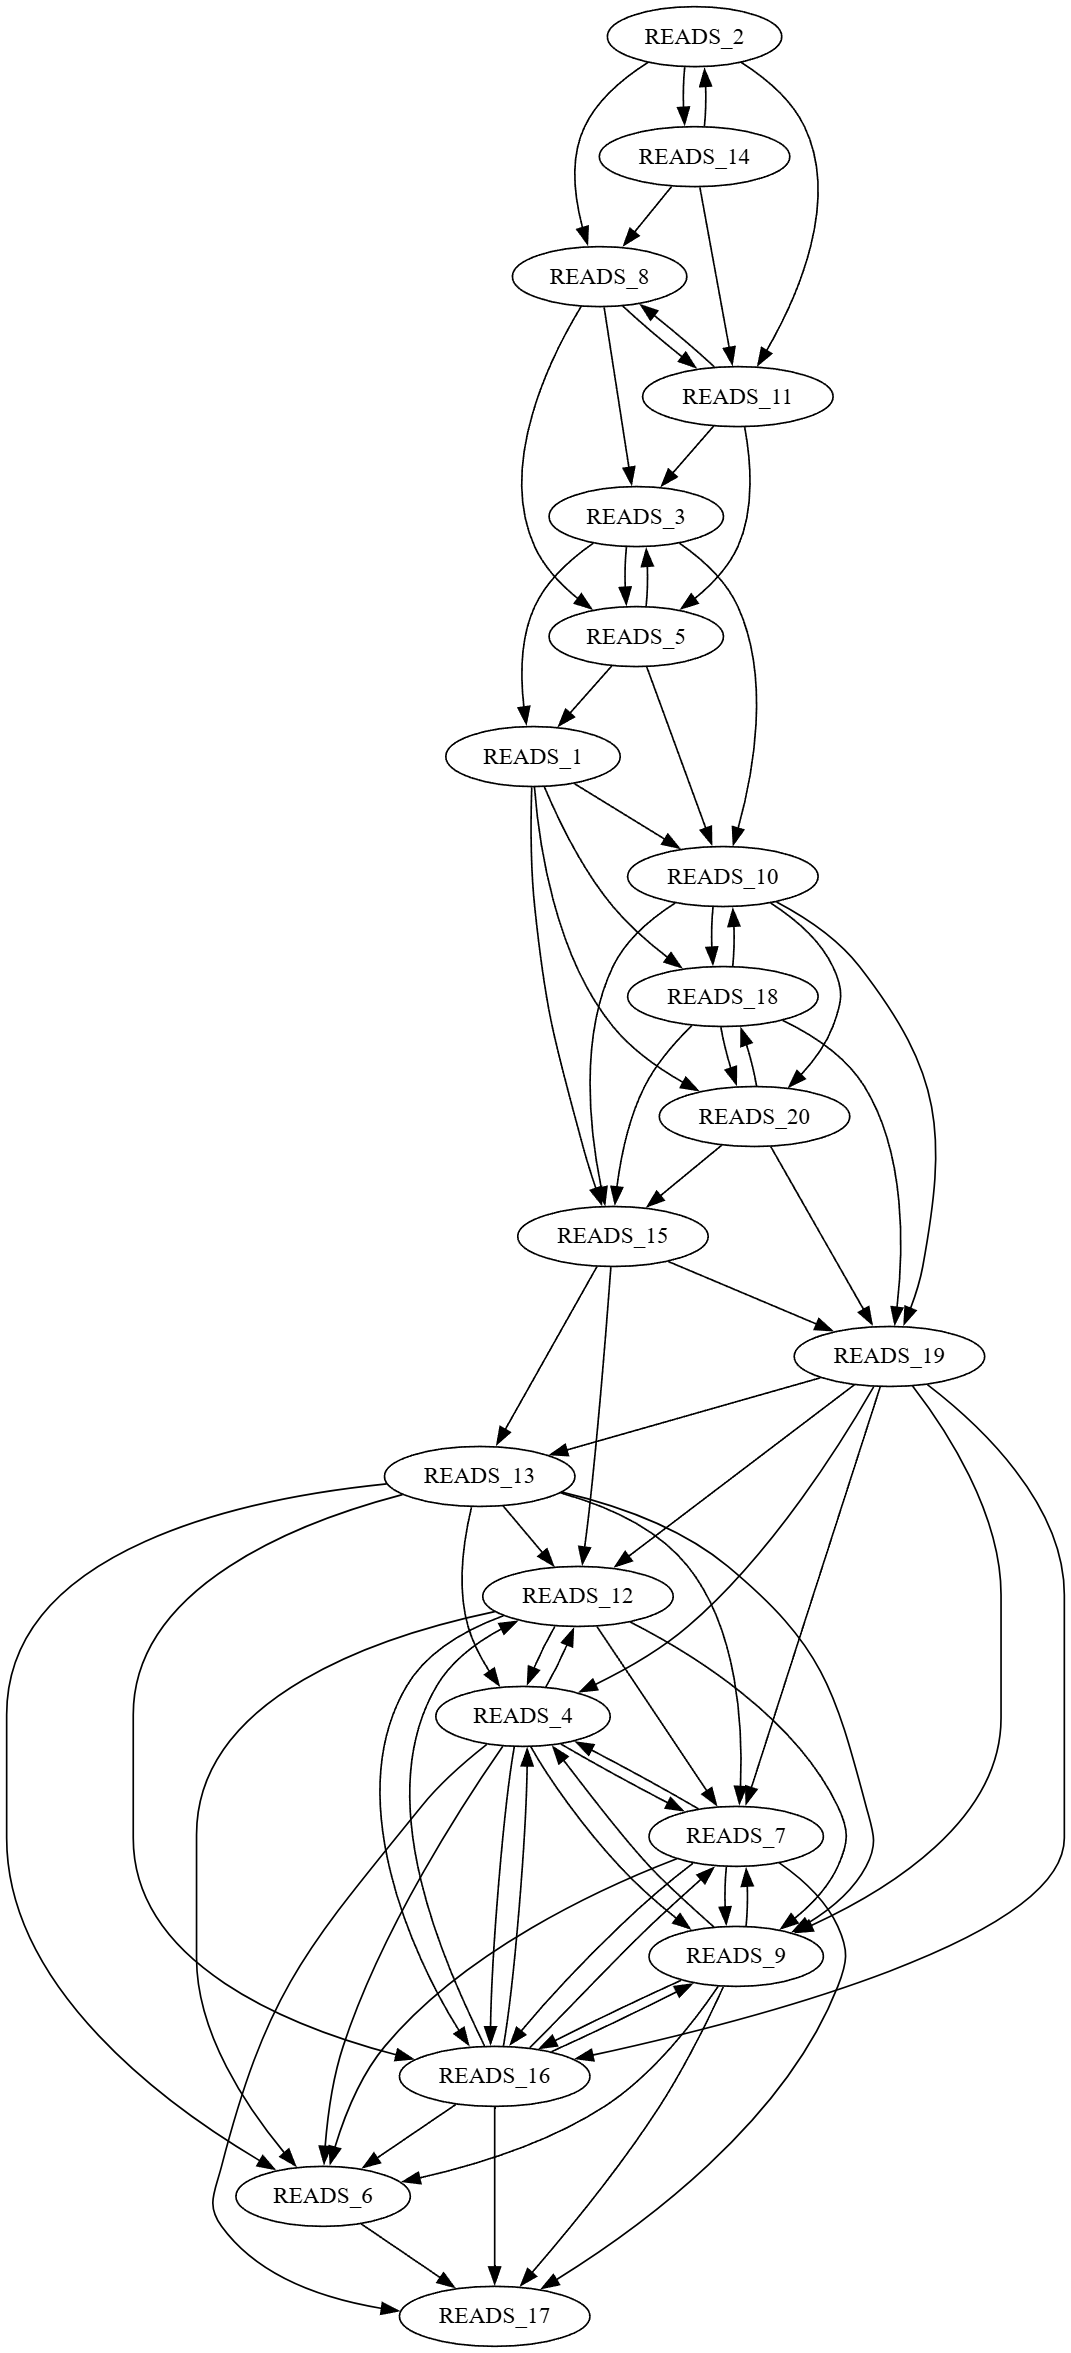
\includegraphics[height=0.75\textheight]{graphe_filtre.png}
\end{center}

\subsection*{2.2b Réduction transitive}
La réduction se fait en deux étapes :
\begin{enumerate}
\item \textbf{Cycles de deux noeuds.} Quand deux reads ont une arête dans chaque sens, on garde seulement celle
de plus grand score. Par exemple, pour READS\_2 $\leftrightarrow$ READS\_14, on garde READS\_2 $\rightarrow$ READS\_14
(1060) et on enlève READS\_14 $\rightarrow$ READS\_2 (756). Il y a 13 cycles de ce type.
\item \textbf{Arêtes transitives.} On enlève une arête $(u,v)$ s'il existe encore un autre chemin de $u$ à $v$.
Par exemple, READS\_2 $\rightarrow$ READS\_11 est enlevée, car le chemin READS\_2 $\rightarrow$ READS\_14
$\rightarrow$ READS\_11 existe déjà. On enlève ainsi 44 arêtes.
\end{enumerate}
Il reste 19 arêtes qui forment un seul chemin passant par les 20 reads, ce qui donne l'ordre :
\begin{center}
READS\_2, 14, 11, 8, 3, 5, 1, 10, 18, 20, 15, 19, 13, 12, 16, 4, 9, 7, 6, 17
\end{center}
Le graphe réduit ci-dessous a été généré avec GraphvizOnline (\url{https://dreampuf.github.io/GraphvizOnline}) ;
l'étiquette de chaque arête est la longueur du chevauchement entre les deux reads.

\begin{center}
\begin{minipage}[c]{0.55\textwidth}\centering\small
\begin{tabular}{lrr}\toprule
Paire consécutive & Score & Chevauchement (nt)\\\midrule
READS\_2 $\rightarrow$ READS\_14 & 1060 & 281 \\
READS\_14 $\rightarrow$ READS\_11 & 492 & 135 \\
READS\_11 $\rightarrow$ READS\_8 & 1072 & 292 \\
READS\_8 $\rightarrow$ READS\_3 & 644 & 169 \\
READS\_3 $\rightarrow$ READS\_5 & 1016 & 280 \\
READS\_5 $\rightarrow$ READS\_1 & 500 & 133 \\
READS\_1 $\rightarrow$ READS\_10 & 804 & 225 \\
READS\_10 $\rightarrow$ READS\_18 & 904 & 258 \\
READS\_18 $\rightarrow$ READS\_20 & 1004 & 277 \\
READS\_20 $\rightarrow$ READS\_15 & 908 & 243 \\
READS\_15 $\rightarrow$ READS\_19 & 632 & 174 \\
READS\_19 $\rightarrow$ READS\_13 & 732 & 199 \\
READS\_13 $\rightarrow$ READS\_12 & 860 & 247 \\
READS\_12 $\rightarrow$ READS\_16 & 996 & 281 \\
READS\_16 $\rightarrow$ READS\_4 & 1032 & 276 \\
READS\_4 $\rightarrow$ READS\_9 & 1068 & 293 \\
READS\_9 $\rightarrow$ READS\_7 & 1044 & 283 \\
READS\_7 $\rightarrow$ READS\_6 & 720 & 194 \\
READS\_6 $\rightarrow$ READS\_17 & 672 & 174 \\
\bottomrule\end{tabular}
\end{minipage}\hfill
\begin{minipage}[c]{0.3\textwidth}\centering
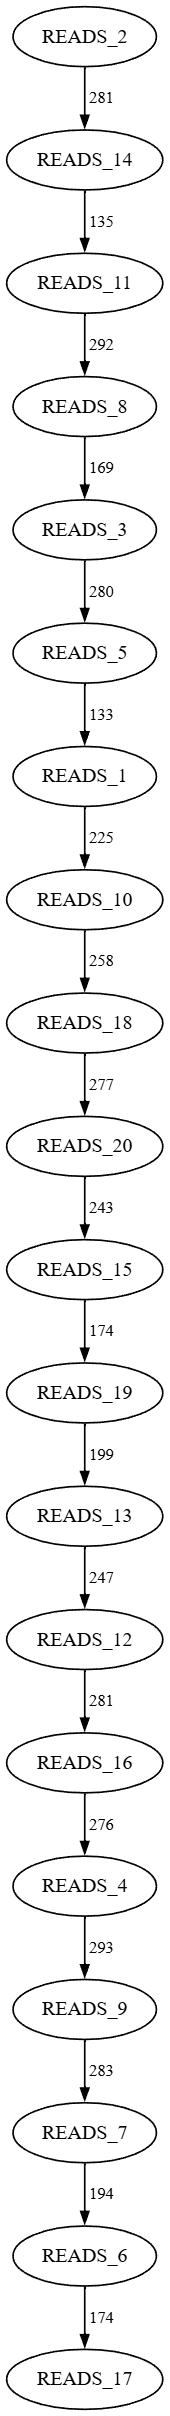
\includegraphics[height=0.62\textheight]{graphe_reduit.png}
\end{minipage}
\end{center}

\subsection*{2.2c Séquence du fragment}
On écrit READS\_2 au complet, puis pour chaque read suivant on ajoute seulement la partie qui dépasse le
chevauchement. En cas de mismatch dans le chevauchement, on garde la base du read précédent.
La longueur est $20\times 300 - 4414 = \mathbf{1586}$ nucléotides (aussi dans \texttt{fragment.fasta}).
\begin{Verbatim}[fontsize=\small]
CTAGGGACTTGGAGAACACAAGTATTATGAAAAGTACTGATGAAAGTTATTAACAGGTTTCGAAAAATAACTTTACTATC
TGACGTGTTGCTTCTGCCGAGGATGACCGTTATTCCTGGTTTTGCATTTATATTTCACGTATGGTTAAATGTGCCAGCGT
TGTGGTTTAAAACTAATAGTAATAATATGCTTCTTTGTTCAGTTGGCTAGAGATTTACTACATCCGTCCTTGGAAGAGGA
AAAGAAAAAACATAACAAGAAACGCCTAGTACAAAGTCCAAATTCTTACTTTATGGATGTAAAATGTCCAGGTAAAATTT
GAAATCTTAATTCCTTTACTAAAGAAAATTTCTGTAGGGATTGCTAGTGTGGTGTGTATAGTTAAGATACATTAGAATCC
TCTGTTGAGTAGAAGTGGGATTACAGAATTGGACATGTCAGGGACAATTTCATAATAAATGTACTGAAACCATTGTAGAA
ACATTTCGGGGTAAGTGAAAACAGGCATTCAAAGTAGATATGCCATTTGAGTGCACTTGTGGCTAATCAAACTGTGGATA
CTCAAAATAGAGATGTTCTTTAATTGTAAAATCCTCACTGGATTTTGACGATGTAGCACAGAAAAAAAATACATTGATTA
CACTGTTTTTAAAAAATTTTGTGTCGCTGCTAGAAAAGTTTAAGTTACACATGTGGCTTGGTGTTTCATAGCACTGAAGT
TACTGATTTTTTTACATATTACCAGAAATGTCGAACAGGTGCTGTTTTCCTCTGCTTTTCATTTTTAAGATTGCCTTTTT
TTTTTTTTAGGTTGCTACAAGATCACCACGGTTTTCAGCCATGCTCAGACTGTGGTTCTTTGTGTAGGTTGTGCAACAGT
GTTGTGCCAGCCTACAGGAGGAAAGGCCAGACTCACAGAAGGTATATCATTTGGCATTCTCCAACCCAGTGATGAGATTG
ATGATTTTAAATGTCTCTATATTAACTGAAAAGTTTAAAGAAATCTTAATGATTCCCAAAATAACTTATCTCACACTGGA
AGAGTTCAAGTGGATTGGCAGCAAATCTGAGATCTATTTGGTGTGACCTGGTGAGATCTAAATATGGAGTCAGCACATGA
TTTTTTTAAGAGTAATATTGCTAAGTAATATTGCTAAGTATCGTCTGAAAATACCTCTAATCAAAATTATTTACTTGAGA
AAAGTATTCAGAATAGTTCCTAAAAATTAATAGTATATTTCTGGTATATAAGCATAAATAATCTGTATATGAGTATTAAT
CCAATATTCTTAAAACTTCAGTATTTTACTTAAAAGTACTATTTGTCATTAAAATTATACCAAAGGTAGAATGCACTTGT
TTAATATACTCTCATGATTCTTTTGCAGGGTGTTCATTTAGAAGAAAGCAACACTAATGATTCAAACAGCTTCCTGAATT
TTAATTTTGTGTTGTCTCTCAGAAAGCCTTATCATAAATTCCATAATTCTAATTAATTTACCAAGATAATGTCATTACAT
TTGGTTATGTAAGTTATACAGCAGTAATCTCCTATTTTGGTGTCAGTTTTTCACTAAAGTTTTTAT
\end{Verbatim}

\section*{3. Recherche d'introns et Blast}
\subsection*{1a. Cadre de lecture}
On a traduit \texttt{sequence.fasta} dans les trois cadres de lecture avec le code génétique standard. Le début de la
protéine (\texttt{MCQRCGLKL...}) apparaît dans le \textbf{cadre 2} : le codon start ATG est aux positions 200 à 202.

\subsection*{1b. Algorithme de programmation dynamique}
On aligne la protéine $P[1..m]$ avec la séquence génomique $S[1..n]$ lue codon par codon : $T(j)$ est l'acide aminé
codé par $S[j..j+2]$. Dans un exon, chaque acide aminé correspond à exactement un codon ; on permet les mismatchs
(coût $\mu=1$) mais pas les indels. Un intron est un saut entre deux codons non consécutifs. Comme on veut minimiser
les introns, on donne un coût constant $\rho$ (ici 3) à chaque intron, peu importe sa longueur (pondération
constante des gaps vue en cours).

$A(i,j)$ = coût minimal pour aligner $P[1..i]$ avec l'acide aminé $i$ sur le codon qui commence en $j$.
\begin{itemize}
\item \textbf{Conditions initiales :} $A(1,j)=\mu(P[1],T(j))$ pour tout $j$, car la région avant le gène ne coûte rien.
\item \textbf{Récurrence :}
\[
A(i,j)=\mu(P[i],T(j))+\min\Big(\underbrace{A(i-1,j-3)}_{\text{même exon}},\ \underbrace{\rho+\min_{k\le j-4}A(i-1,k)}_{\text{nouvel intron}}\Big)
\]
Le premier cas continue l'exon avec le codon juste avant ; le second ouvre un intron entre le codon $k$ et le codon $j$.
En gardant le minimum courant de la ligne $i-1$, chaque case se calcule en $O(1)$, donc l'algorithme est en $O(mn)$.
Si on impose que tous les exons soient dans le même cadre, on prend seulement les $k\equiv j \pmod 3$.
\item \textbf{Chemin :} la meilleure valeur est $\min_j A(m,j)$. On remonte les pointeurs : un pas $j\to j-3$ reste dans
le même exon, un saut $j\to k$ correspond à un intron.
\end{itemize}
\subsection*{2. Blastp}
On a soumis la séquence de \texttt{geneX.fasta} à Blastp (NCBI). Le meilleur alignement est avec la protéine
\textbf{40S ribosomal protein S27-like} (\emph{small ribosomal subunit protein eS27-like}, gène \textbf{RPS27L}) :
82 acides aminés identiques sur 82 (100\,\%), sans gap, avec une E-value de $9\times10^{-56}$. L'alignement couvre les
positions 19 à 100 de la protéine X ; seuls les 18 premiers acides aminés ne sont pas alignés. Les premiers résultats
sont la même protéine chez plusieurs mammifères (rat, bœuf, \dots), ce qui montre qu'elle est très conservée.

\begin{center}
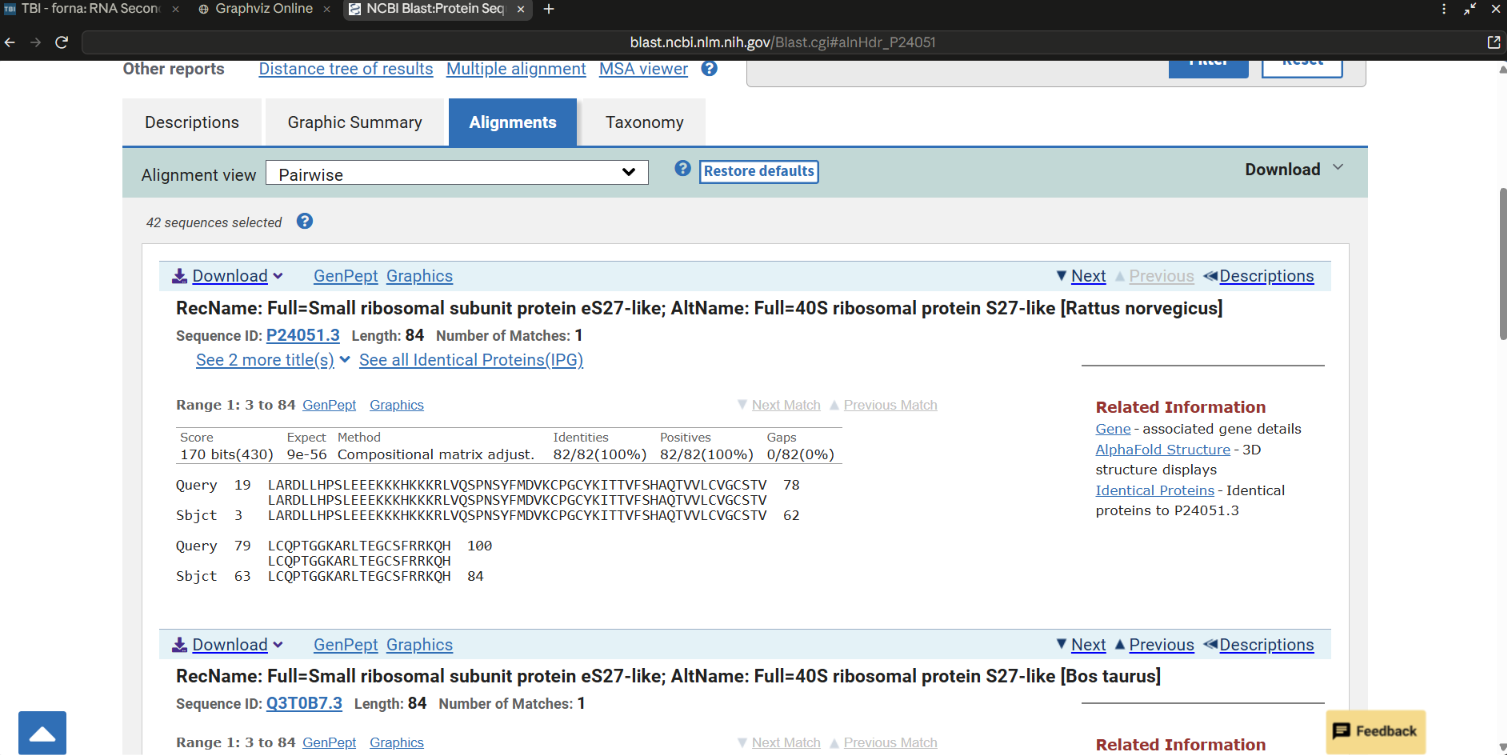
\includegraphics[width=\textwidth]{blastp.png}
\end{center}

\textbf{Fonction :} RPS27L est une protéine ribosomique de la famille de RPS27 (petite sous-unité 40S du ribosome).
Son gène est une cible directe de p53 : elle est produite après des dommages à l'ADN, favorise l'apoptose et participe
à la régulation de l'axe p53--MDM2.

\section*{4. Repliement d'ARN}
\subsection*{Q7. Repliement 2D}
\begin{center}
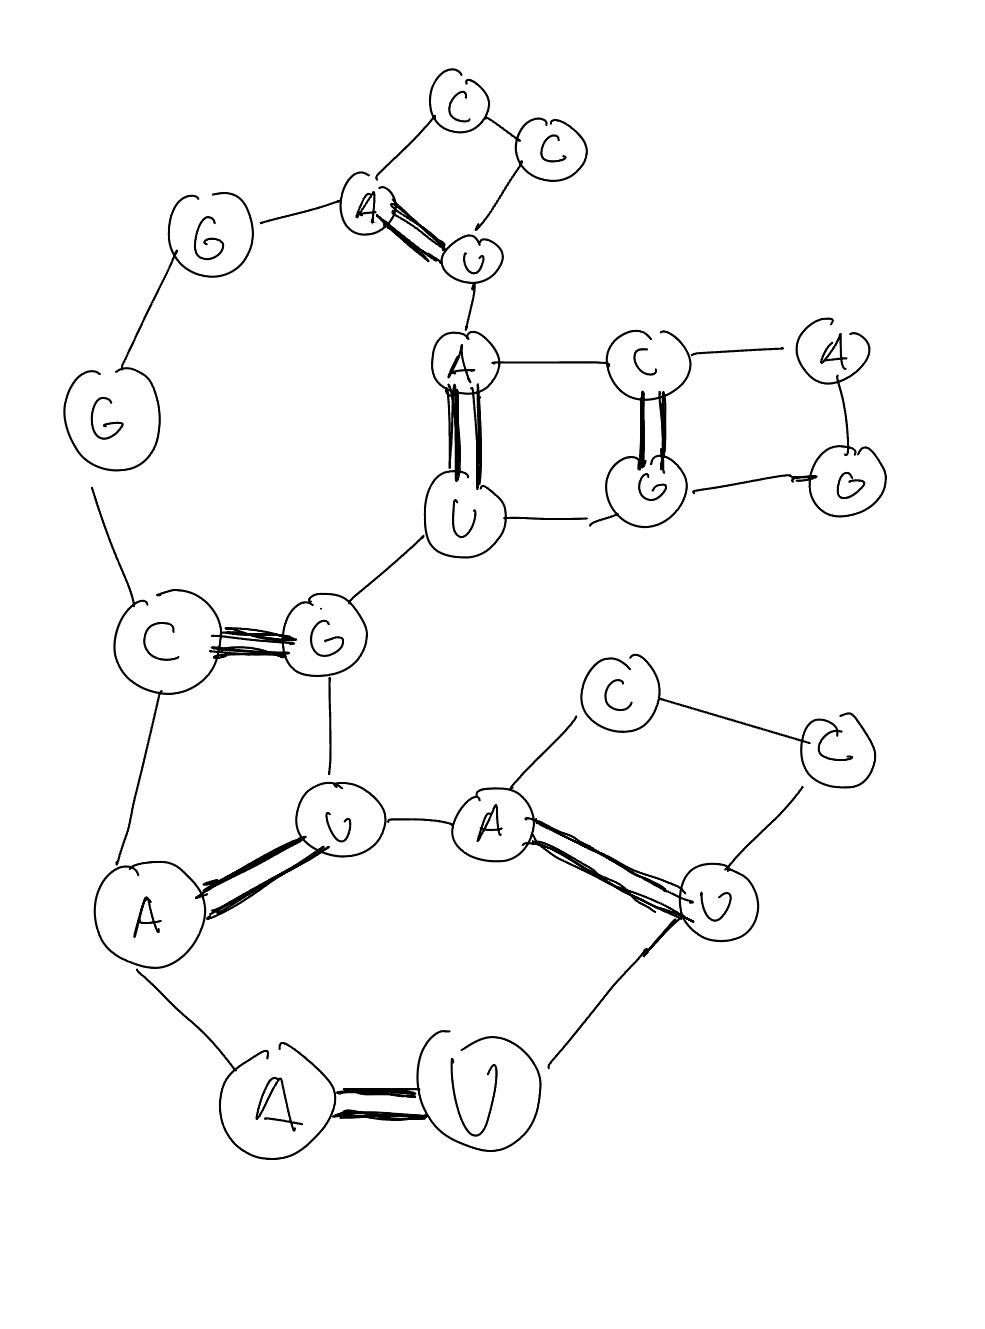
\includegraphics[width=0.45\textwidth]{repliement_main.jpg}
\end{center}

\subsection*{Q8 (bonus). Maximiser le nombre d'empilements en $O(n^3)$}
Un empilement est une paire $(i,j)$ telle que $(i+1,j-1)$ est aussi appariée. On adapte l'algorithme de Nussinov
avec deux tables ($p(x,y)=1$ si $x$--$y$ est A--U ou G--C) :
\begin{itemize}
\item $D(i,j)$ : nombre maximal d'empilements pour $S[i..j]$ ;
\item $E(i,j)$ : même chose, mais en imposant que $i$ et $j$ soient appariés ($-\infty$ si $p(S_i,S_j)=0$).
\end{itemize}
\textbf{Conditions initiales :} $D(i,i)=D(i,i-1)=0$ et $E(i,j)=0$ si $j-i\le 1$.

\textbf{Récurrences :}
\[
E(i,j)=\max\begin{cases}
D(i+1,j-1) & (i,j) \text{ n'est pas empilée}\\
E(i+1,j-1)+1 & \text{si } p(S_{i+1},S_{j-1})=1 \text{ (empilement)}
\end{cases}
\]
\[
D(i,j)=\max\begin{cases}
D(i+1,j) & i \text{ non apparié}\\
D(i,j-1) & j \text{ non apparié}\\
E(i,j) & i \text{ apparié avec } j\\
\max_{i+1\le k\le j-2}[D(i,k)+D(k+1,j)] & \text{bifurcation}
\end{cases}
\]
On remplit diagonale par diagonale et la réponse est $D(1,n)$. Pour retrouver le repliement, on part de $D(1,n)$
et on regarde quel cas a donné la valeur : dans $E$ on note la paire $(i,j)$, et une bifurcation donne deux
sous-intervalles à traiter (avec une pile). Il y a $O(n^2)$ cases et la bifurcation coûte $O(n)$ par case, donc
l'algorithme est en $O(n^3)$ en temps et $O(n^2)$ en espace.

\end{document}
